Plusieurs systèmes ont été étudiés afin d'incorporer le capteur dans une conception permettant de connecter les membranes et le corps de chauffe
ainsi que d'y attacher un système apportant un flux d'air (imitation de la respiration du patient).

\section{Design 1}
\begin{figure}[H]
    \centering
    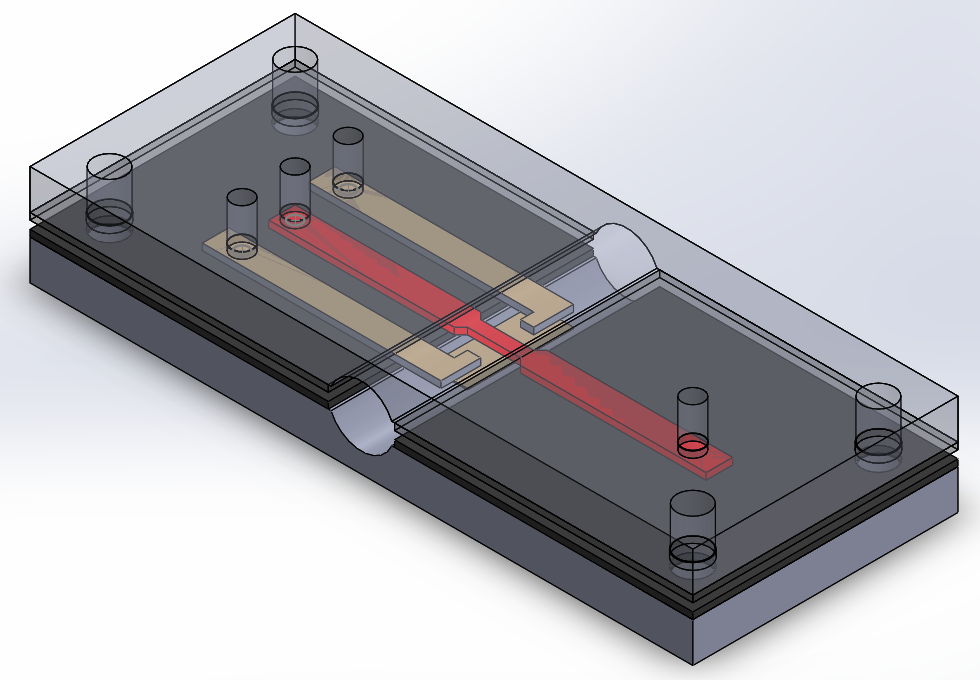
\includegraphics[scale = 0.5]{images/Design1.png}
    \caption{Design 1}
    \label{fig:design1}
\end{figure}
Ce premier design est le plus basique. Il vient plaquer le capteur entre deux couches presque symétriques. Sur une des couche se trouvent des
perçages permettant de tenir des contacts à ressorts (pointes ressorts). Celles-ci viennent s'appuyer sur le capteur afin d'assurer les contacts
électriques. Un joint plat peut venir des deux côtés du capteur afin d'assurer l'étanchéité du système.\\
Cette solution a le désavantage d'avoir une arrivé d'air scindée en deux. Le placement ainsi que l'étanchéité au niveau de l'entrée
arrondie risque d'être mauvaise. \\
Ceci mis de côté, c'est une solution simple, rapide et compacte.

\section{Design 2}
Afin d'éviter l'entrée d'air scindée en deux, une solution pourrait être celle représentée ci-dessous :
\begin{figure}[H]
    \centering
    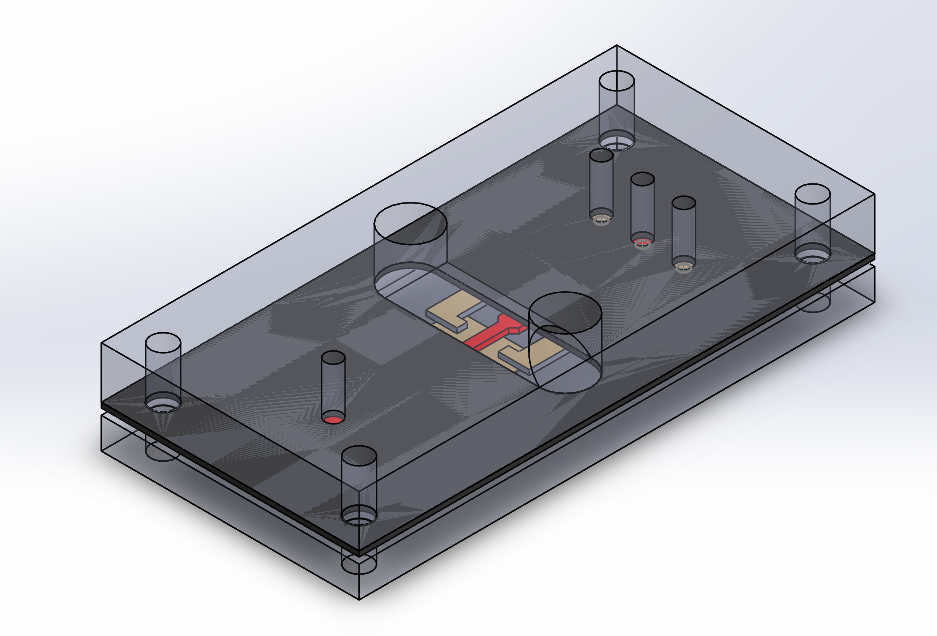
\includegraphics[scale = 0.5]{images/Capteur_design2_caoutch.png}
    \caption{Design 2}
    \label{fig:design2}
\end{figure}
L'arrivée d'air se fait par le haut du système et est dévié par la suite afin d'arriver sur le capteur. Cette solution permet d'avoir une
entrée d'air plus régulière et utilisable que la solution précédente. Cependant, elle ajoute un risque non-négligeable au niveau des turbulences. En effet,
les coudées risquent d'engendrer des turbulences au niveau du flux qui pourraient altérer les résultats.

\section{Design 3}
Une manière de diminuer ces turbulences seraient d'élargir le système afin que les coudées ne se retrouvent pas trop proches de la
membrane.

\begin{figure}[H]
    \centering
    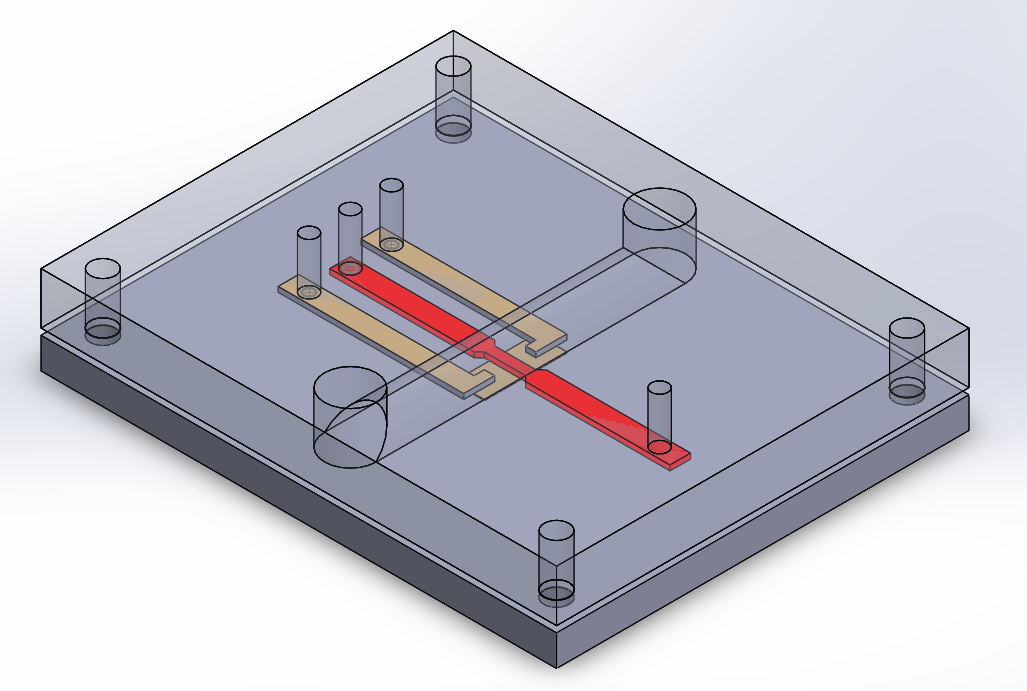
\includegraphics[scale = 0.5]{images/Design4}
    \caption{Design 5}
    \label{fig:design4}
\end{figure}

\subsection{Design 4}
Une autre manière d'éviter ce problème de turbulences et de changer la conception. Ainsi, le capteur pourrait être fabriqué selon la
figure \ref{fig:design6}.

\section{Design 4}
\begin{figure}[H]
    \centering
    \includegraphics[scale = 0.5]{images/Design6}
    \caption{}
    \label{fig:design6}
\end{figure}

Cependant cette solution engendre un nombre de pièces plus élevé que les designs précédents. En effet, pour un conception comme celle
de la figure \ref{fig:design6}, 4 pièces seraient nécessaires contre 2 pièces pour les solutions précédentes.\\
Deux pièces viendraient pincer le capteur en sandwich comme montré pour le design 1, figure \ref{fig:design1}, puis, deux autres pièces
viendraient se poser sur les deux longueurs du système afin de permettre de conncter facilement une arrivée d'air.

\section{Design 5}
Finalement, une dernière conception a été imaginée :

\section{Design 5}
\begin{figure}[H]
    \centering
    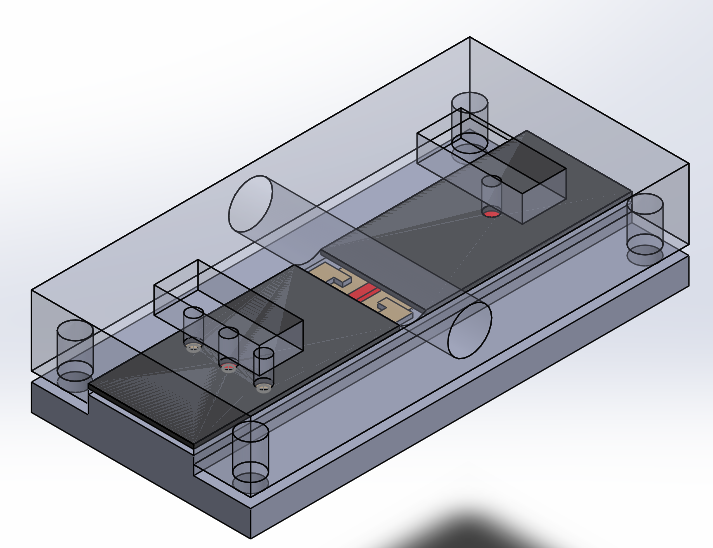
\includegraphics[scale = 0.5]{images/Design5_int_caoutch.png}
    \caption{}
    \label{fig:design5}
\end{figure}

Cette dernière permettrait de garder une solution à deux pièces seulement et incorporerait une entrée et une sortie d'air facilitée.
La membrane (capteur) posée sur une première pièce légèrement surrélevée. Un joint plat d'échantéité viendrait sur la membrane (en noir
sur la figure). Puis, une seconde pièce viendrait s'appuyer en sandwich contre le joint et le capteur. Cette pièce, sur le dessus, est
percée afin d'amener le flux d'air au niveau du capteur. Des plus petits perçages ainsi que des espaces creusés dans la pièce du dessus
permettent aux pointes ressorts de venir se poser sur la membrane afin d'assurer la connection électrique.
\begin{comment}
\end{comment}